---
title: |
 ![](../../man/figures/NMdata_logo_v01.png){width=1in}\linebreak
 NMdata: A fast R package for efficient data preparation, consistency-checking and post-processing in PK/PD modeling
author: Philip Delff
date: June 2022
fontsize: 8pt
header-includes:
 - \usepackage{adjustbox}
output: 
 beamer_presentation:
  slide_level: 2
  keep_tex: true
classoption: "aspectratio=169"
---

<!-- TODO: -->
<!-- Motivation -->
<!-- Describe testing framework -->
<!-- Pretty up -->
<!-- Tools for programming -->
<!--  - egdt -->
<!--  - findCovs -->
<!--  - findVars -->
<!--  - NMreadSection -->
<!--  - NMextractText -->

<!-- listMissings -->
<!-- cc, cl -->
<!-- update flagsAssign and flagsCount -->
<!-- NMcheckData -->
<!-- NMwriteSection made easier -->
<!-- NMscanMultiple -->
<!-- tracee -->
<!-- execSafe -->



<!-- Supposedly this chunk option should activate a profile but it doesn't work -->
<!-- ,class.source="smaller" -->


## Outline
\tableofcontents[hideallsubsections]


# Introduction

## What is NMdata?
::: columns
:::: column
### NMdata is 

An R package that can help

*  Creating and checking event-based data sets for PK/PD modeling
*  Keeping Nonmem code updated to match contents of datasets
*  Read all output data and combine with input data from Nonmem runs
- supply output list file (.lst), and the reader is very flexible and automated 

Designed to fit in to the user's setup and coding preferences

* NMdata comes with a configuration tool that can be used to tailor default behaviour to the user's system configuration and preferences.

::::

:::: column

### NMdata is not

* A plotting package

* A tool to retrieve details about model runs

* A calculation or simulation toolbox

* A "silo" that requires you to do things in a certain way
- No tools in NMdata requires other NMdata tools to be used

::::
:::

$$\vspace{.01in}$$

* The data creation tools should be relevant independently of estimation/simulation tool.
* Latest stable release is 0.0.12 and is available on CRAN and MPN (starting from 2022-06-15 snapshot).

## NMdata 0.0.12 on MPN
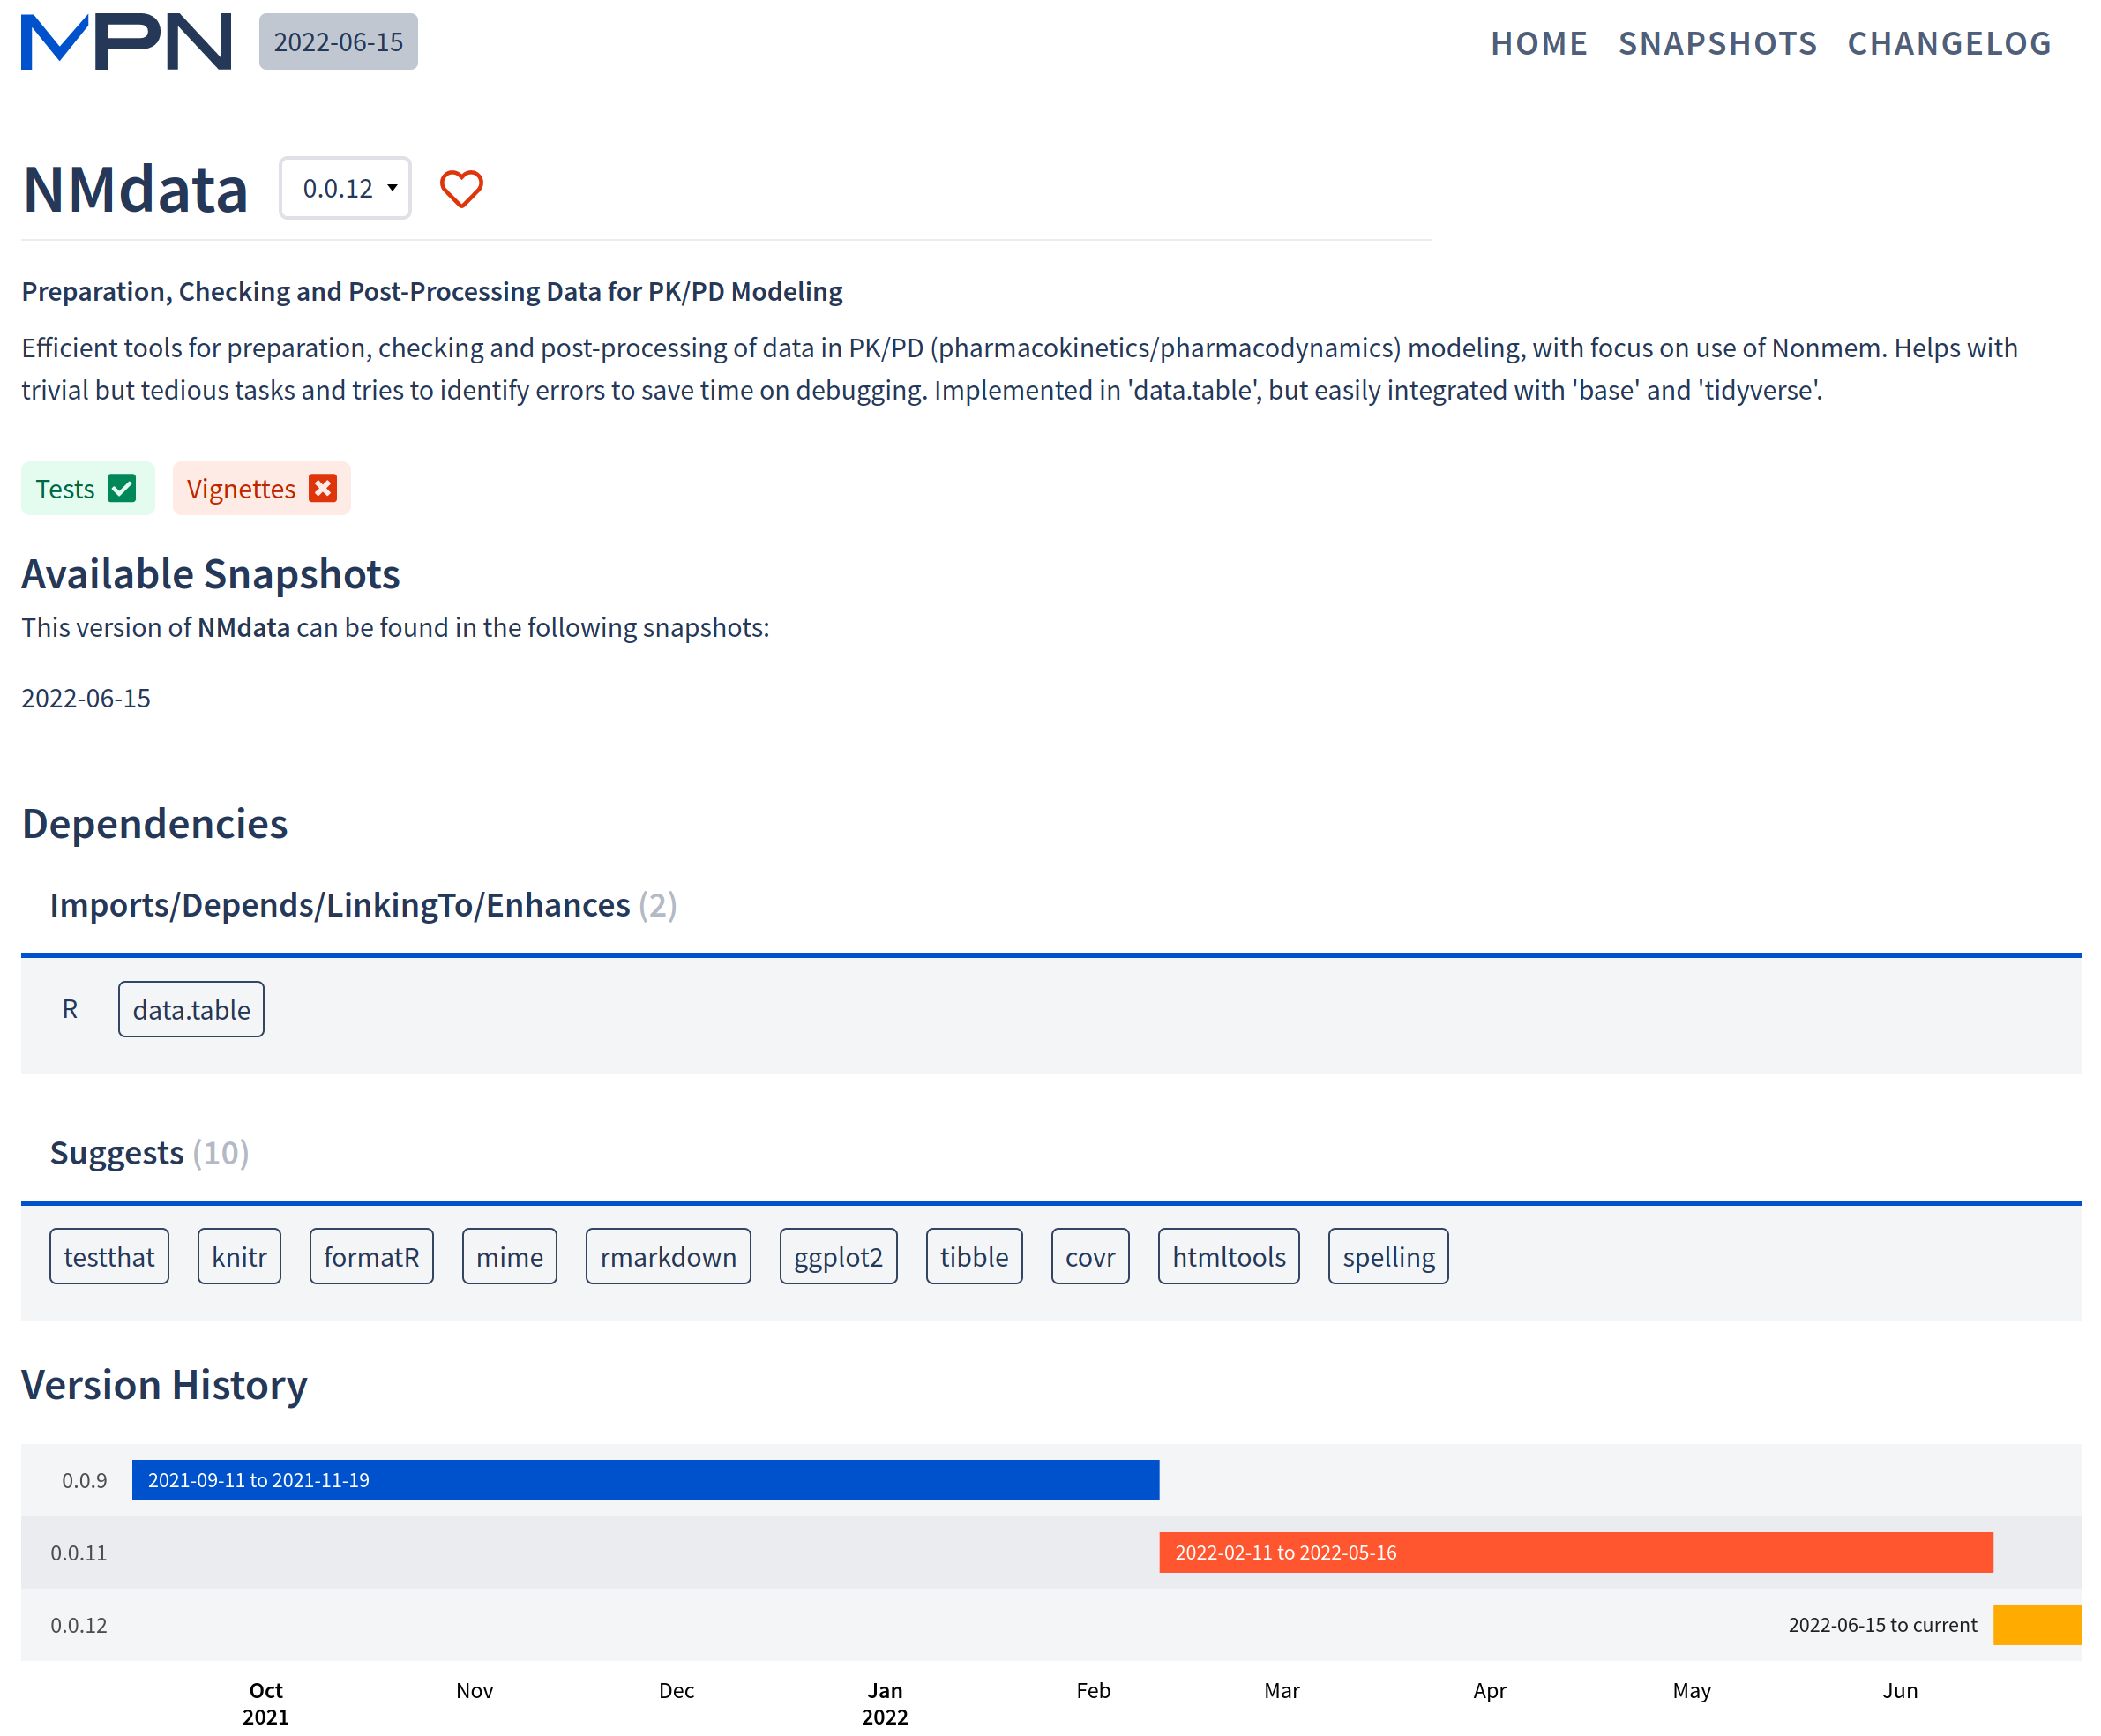
\includegraphics[width=3.5in]{figures/nmdata_mpn_2022-06-27 22-03-35.png}


<!-- ## Who can find NMdata useful? -->

<!-- * The data set creation tools are relevant no matter the estimation and simulations tools. -->

<!-- * Nonmem users will find additional tools for handling the exchange of data between R and Nonmem. -->


<!-- ## About the author -->
<!-- * Pharmacometrician with experience from biostatistics -->

<!-- * Background in engineering, experience as system administrator, 15 years of R experience -->

<!-- * Very concerned with code robustness and ensuring data consistency. -->

<!-- * Authored an R package on safe data transfer from SAS to R and one on survival analysis.  -->

<!-- I hate being stuck in leg work and having too little time for modeling, -->
<!-- reflection, and understanding key questions. `NMdata` is a big help for -->
<!-- me personally in freeing time to more high-level tasks. -->


<!-- Lots of work missing on this one -->
<!-- ## Motivation -->

<!-- PK/PD modeling is technically extremely heavy. We want to do provide clarity to decision making, but spend a lot of our time in deep mud. -->

<!-- `NMdata` is my humble experience collected in efficient functions that fill some holes and help with some of the most annoying design -->

## How to update to recent MPN snapshot
Update the `pkgr.yml` file: 
(example: `prod_vx123_001_analysis/trunk/analysis/vx_123_001_project/pkgr.yml`)

```
Version: 1
Threads: 1
Packages:
  - NMdata

# this will allow packages to be cached across projects for faster installs on new projects
Cache: /data/prod_vx708_001_pkgcache-2022-06-15
Repos:
  - MPN: https://mpn.metworx.com/snapshots/stable/2022-06-15
Lockfile:
    Type: renv
```
Then go to `prod_vx123_001_analysis/trunk/analysis/vx_123_001_project` and install/update packages from the linux terminal (not R):
```
$ cd /data/prod_vx123_001_analysis/trunk/analysis/vx_123_001_project
$ pkgr --update install
```

## Motivation
* The workflow of a pharmacometrician is very technical, with many risks of errors.

* Technical workload takes time from modeling, reflection, and
understanding key questions. 

* During the first 2-3 years I spent in pharmacometrics, I must have spent half the time coding, desparately trying to get Nonmem to behave, and to understand the properties of the estimates I obtained.

* Most of us develop our own ways to avoid some of the many
difficulties in this process. This takes a lot of time and is most
often only because we don't have adequate tools at hand. Or don't know them.

* I generalized some of my solutions and collected them in `NMdata`.

* Almost every single line of code in the package is motivated by bad
experiences. Errors, fear of errors, time wasted on debugging and
double checking.

* I have no intention of missioning these approaches to others. But if
you find something interesting, feel free to take advantage.


<!-- This could become a good slide, but so far not ready at all -->
<!-- ## Overview of NMdata functionality -->
<!-- * Data creation -->
<!-- - Checking of compatibility of data.frames. -->
<!-- - Merge with automated checks  -->

<!-- * Nonmem control stream editing -->

<!-- * Retrieve data from Nonmem -->




## Getting started
Install from `CRAN` or from `MPN` using `pkgr`.

```r
library(NMdata)
```

```
## Welcome to NMdata. Best place to browse NMdata documentation is
## https://philipdelff.github.io/NMdata/
```






Three vignettes are available so far (see "Vignettes" tab when visiting URL above):

* [Cheat sheet](https://htmlpreview.github.io/?https://github.com/philipdelff/NMdata/blob/master/vignettes/NMdata-cheat.html)
* [Data creation tools](https://philipdelff.github.io/NMdata/articles/DataCreate.html)
* [Automated and general reader of Nonmem data](https://philipdelff.github.io/NMdata/articles/NMscanData.html)
* [FAQ](https://philipdelff.github.io/NMdata/articles/NMdata-FAQ.html)

<!-- dplyr users, please see FAQ for how to make all NMdata functions return tibbles. -->

For a quick overview (after installation), do:

<!-- Would be good to show a truncated output here -->

```r
help(package="NMdata")
```

All functions and their arguments are documented in ?manual pages.

<!-- prepare example data behind the scenes -->


# Data set creation


## Compare compatibility of data sets for rbind and merge: `compareCols`

::: columns
:::: column

* In order to rbind or merge data sets, they must be compatible in 
- presence of columns, depending of desired outcome
- equally importantly, the classes of the common columns.
* `compareCols` provides an overview of these properties for any number of data sets. 
- By default, only discrepancies are returned. 
- Using `diff.only=FALSE` will give the complete list of columns in the two datasets.

A slightly modified version of the `pk` dataset has been created.

* Rows have been omitted
* `CYCLE` has been removed, and
* `AMT` has been recoded to character



:::: 
:::: column



```{.r .smaller}
compareCols(pk,pk.reduced)
```

```
## Dimensions:
```

```
##          data nrows ncols
## 1:         pk  1502    22
## 2: pk.reduced   751    21
```

```
## 
## Columns that differ:
```

```
##    column      pk pk.reduced
## 1:  CYCLE integer       <NA>
## 2:    AMT integer  character
```

```
## 
```

```
## Columns where no differences were found: BLQ,
## CMT, DOSE, DV, EVENTU, EVID, FLAG, ID, NAME,
## NOMTIME, PART, PROFDAY, PROFTIME, STUDY, TIME,
## TIMEUNIT, TRTACT, WEIGHTB, eff0, flag.
```


\vspace{12pt}

Before merging or stacking, we may want to 

* recode `AMT` in one of the datasets to get the class we need
* decide what to do about the missing `CYCLE` in one of the datasets 

::::
:::

## Keep track of missing values

```r
missings <- listMissings(pk)
```

```
##    variable Nmissing
## 1:       DV      150
```

```r
head(missings)
```

```
##    variable row value
## 1:       DV   1  <NA>
## 2:       DV  11  <NA>
## 3:       DV  21  <NA>
## 4:       DV  31  <NA>
## 5:       DV  41  <NA>
## 6:       DV  51  <NA>
```

You can specify 

* What columns to search
* A grouping variable for findings (i.e. study if combining datasets) 
* The strings that are interpreted as missing. 

From `?listMissings`:
```
Usage:

     listMissings(data, cols, by, na.strings = c("", "."), quiet = FALSE, as.fun)
```


<!-- %%% renameByContents.R -->
## Rename columns based on contents
::: columns
:::: column 
### renameByContents
* Nonmem almost entirely relies on numeric data values.
* The source data
will often contain character variables, i.e. columns with non-numeric
data values. We want to use these and other non-numerics in post-processing.
* If the column names reflect whether the values are numeric, mistakes and double-checking can be avoided. 
* `renameByContents` renames columns if a function of their contents returns `TRUE`.

### `NMisNumeric`

- `NMisNumeric` is a function that tests if the contents are numeric to `Nonmem`. 
- Subject ID `"1039"` (character class) will be a numeric in Nonmem, `"1-039"` will not. 
- We invert that, and those that Nonmem cannot interpret as numeric become lowercase. 

:::: 

:::: column
All column names are capital case. We rename to lowercase those that Nonmem will not be able to interpret as numeric.
\footnotesize



```r
pk <- renameByContents(data=pk,
                       fun.test=NMisNumeric,
                       fun.rename = tolower,
                       invert.test = TRUE)
```

`compareCols` shows that four columns were renamed:


```r
compareCols(pk.old,pk)
```

```
## Dimensions:
```

```
##      data nrows ncols
## 1: pk.old  1502    22
## 2:     pk  1502    22
```

```
## 
## Columns that differ:
```

```
##      column    pk.old        pk
## 1:   EVENTU character      <NA>
## 2:     NAME character      <NA>
## 3: TIMEUNIT character      <NA>
## 4:   TRTACT character      <NA>
## 5:   eventu      <NA> character
## 6:     name      <NA> character
## 7: timeunit      <NA> character
## 8:   trtact      <NA> character
```

```
## 
```

```
## Columns where no differences were found: AMT, BLQ, CMT,
## CYCLE, DOSE, DV, EVID, FLAG, ID, NOMTIME, PART, PROFDAY,
## PROFTIME, STUDY, TIME, WEIGHTB, eff0, flag.
```
\normalsize
::::

:::

<!-- %%% list additional small function -->
<!-- %% dims -->

## Automated checking of merges

* Merges are a very common source of data creation bugs. 
* Merges likely leave you with an unexpected number of
rows, some repeated or some omitted. 
* `mergeCheck` is a wrapper of `merge` 
which only accepts the results if 

**The rows that come out
of the merge are the exact same as in one of the existing datasets,
only columns added from the second dataset**

* This limitation of the
scope of the merge allows for a high degree of automated checks of
consistency of the results.

* This is not to say that merges beyond the scope of `mergeCheck` are
relevant or necessary. But if `mergeCheck` covers your needs, it's a
real time saver in terms of automated checks.

**mergeCheck is not a new implementation of merge. It's an implementation of checks.**

* `mergeCheck` uses `merge.data.table`. The contribution is the checks that no rows are lost, duplicated or added. 

* The order of rows in the resulting data is always the same as the first dataset supplied.

Is `mergeCheck` slower?

- If you don't use data.table already, `mergeCheck` is likely to be way faster than what you use already. 
- The checking overlay should be neglegible.
- If checks fail, an additional merge is done to help user identify problems. This may cost significant additional time but is likely to save you coding and (at least) the same calculation time anyway.


## mergeCheck
\framesubtitle{Example: Would your standard checks of merges capture this?}



Say we want to add a covariate from a
`dt.cov`.  We expect the number of rows to be unchanged from `pk`. `mergeCheck` more strictly requires that we get all and only the _same_ rows:

::: columns
:::: column
### Without `mergeCheck`
\footnotesize

```r
## The resulting dimensions are correct
pkmerge <- merge(pk,dt.cov,by="ID")
dims(pk,dt.cov,pkmerge)
```

```
##       data nrows ncols
## 1:      pk  1502    22
## 2:  dt.cov   150     2
## 3: pkmerge  1502    23
```

```r
## But we now have twice as many rows for this subject
dims(pk[ID==31],pkmerge[ID==31])
```

```
##                 data nrows ncols
## 1:      pk[ID == 31]    10    22
## 2: pkmerge[ID == 31]    20    23
```
:::
:::: column
### `mergeCheck` throws an error
...and suggests what is wrong
\footnotesize


```r
try(mergeCheck(pk,dt.cov,by="ID")) 
```

```
## Rows disappeared during merge.
```

```
## Rows duplicated during merge.
```

```
## Overview of dimensions of input and output data:
##    nrows ncols
## 1:  1502    22
## 2:   150     2
## 3:  1502    23
```

```
## Overview of values of by where number of rows in x changes:
##     ID N.x N.result
## 1:  31  10       20
## 2: 180  10        0
```

```
## Error in mergeCheck(pk, dt.cov, by = "ID") : 
##   Merge added and/or removed rows.
```
::::
\normalsize
:::

### Conclusion
If you only want to add columns by a merge, `mergeCheck` does all the necessary checks for you.

## Exclusion flags
\framesubtitle{Keep track of data exclusions - don't discard!}

* It is good practice not to discard unwanted records from a dataset but to flag
them and omit them in model estimation. 

* When reporting the analysis,
we need to account for how many data records were discarded due
to which criteria. 

* The implementation in `NMdata` is based on sequentially checking
exclusion conditions.

* The information is represented in one numerical column for
Nonmem, and one (value-to-value corresponding) character column for
the rest of us.

## FlagsAssign
::: columns
:::: column

* `flagsAssign` applies the conditions sequentially, by increasing or decreasing
value of `FLAG`. 
* You can use any expression that can be evaluated _row-wise_ within
the data.frame. In this case, `BLQ` has to exist in `pk`.
* If you need to evaluate a condition based on multiple rows (say inadequate dosing history for a subject), do that first, and include a column representing this condition.
* `FLAG=0` means that none of the conditions were met and row is kept in analysis. This cannot be customized.
* In `Nonmem`, you can include `IGNORE=(FLAG.NE.0)` in `$DATA` or `$INFILE`.

::::

:::: column
\footnotesize



```r
dt.flags <- fread(text="FLAG,flag,condition
10,Below LLOQ,BLQ==1
100,Negative time,TIME<0")

pk <- flagsAssign(pk,tab.flags=dt.flags,subset.data="EVID==0")
```

```
## Coding FLAG = 100, flag = Negative time
```

```
## Coding FLAG = 10, flag = Below LLOQ
```

```r
pk <- flagsAssign(pk,subset.data="EVID==1",flagc.0="Dosing")
```
::::

:::


## `flagsCount`
* An overview of the number of observations disregarded due to the
different conditions is then obtained using `flagsCount`:

* `flagsCount` includes a `file` argument to save the the table right
away.



\footnotesize

```r
flagsCount(data=pk[EVID==0],tab.flags=dt.flags)
```

```
##                  flag N.left Nobs.left N.discard N.disc.cum Nobs.discard Nobs.disc.cum
## 1: All available data    150      1352        NA          0           NA             0
## 2:      Negative time    150      1350         0          0            2             2
## 3:         Below LLOQ    131       755        19         19          595           597
## 4:       Analysis set    131       755        NA         19           NA           597
```



* Now pick the columns you want and format your table for the report.


# Finalize data for Nonmem 
## Advice: always include a unique row identifier

::: columns
:::: column
### Why
A unique identifier is needed in order to

* Track rows in analysis data back to source data

* Reliably combine (by merge) output with input data

### The identifier should be

* Numeric
- For Nonmem to be able to read it
* Integer
- To avoid risk of rounding
- It is _not_ a problem if represented as a `double` in `R`

* Increasing
- Not strictly necessary
- Avoid confusion
- May be useful for post-processing to have a single column to order by

::::
:::: column

### Sort rows and add a row counter 

* with `data.table`

```r
## order
setorder(pk,ID,TIME,EVID)
## add counter
pk[,ROW:=.I]
```

* Or, with `dplyr` (I'm not very familiar with `dplyr`)

```r
pk <- pk %>%
    arrange(ID,TIME,EVID) %>%
    mutate(ROW=1:n())
```

::::
:::


<!-- *`NMscanData` will most often work even if you don't include a row -->
<!-- identifier. But this will rely on interpretation of Nonmem code. -->

## NMorderColumns
::: columns
:::: column
\vspace{12pt}
* The order of columns in Nonmem is important for two reasons. 

- Non-numeric Characters in a variable read into Nonmem will make the run
fail
- The number of
variables you can read into Nonmem is restricted (may not apply to recent Nonmem versions)

* `NMorderColumns` uses a mix of recognition of column names and analysis of the
column contents to sort the columns. 

- First: Standard columns (`ID`, `TIME`, `EVID` etc.) and usable columns first

- Columns that cannot be converted to numeric are put in the back

- Additional columns to place earlier (argument `first`) or late (`last`) can be specified. 

- See `?NMorderColumns` for more options.

* `NMorderColumns` does not sort rows, nor does it modify any contents of columns.

::::
:::: column
<!-- Use print.data.table to get top and bottom with correct row numbers -->
\footnotesize

```r
pk.old <- copy(pk)
pk <- NMorderColumns(pk,first="WEIGHTB")
```
\normalsize
We may want to add `MDV` and rerun `NMorderColumns`.
\footnotesize

```r
data.table(old=colnames(pk.old),new=colnames(pk))
```

```
##          old      new
##  1:       ID      ROW
##  2:  NOMTIME       ID
##  3:     TIME  NOMTIME
##  4:     EVID     TIME
##  5:      CMT     EVID
##  6:      AMT      CMT
##  7:       DV      AMT
##  8:    STUDY       DV
##  9:      BLQ  WEIGHTB
## 10:    CYCLE     FLAG
## 11:     DOSE    STUDY
## 12:     PART      BLQ
## 13:  PROFDAY    CYCLE
## 14: PROFTIME     DOSE
## 15:  WEIGHTB     PART
## 16:     eff0  PROFDAY
## 17:   eventu PROFTIME
## 18:     name     eff0
## 19: timeunit   eventu
## 20:   trtact     flag
## 21:     FLAG     name
## 22:     flag timeunit
## 23:      ROW   trtact
##          old      new
```
::::
\normalsize
:::


## `NMcheckData`: Check data syntax for Nonmem compatibility 
* Aim: check data for all potential Nonmem compatibility issues and other obvious errors.

* Findings must be returned in a structure so related subsets of the
  data can easily be identified for further inspection. 

::: columns
:::: column
* `NMcheckData` contains a very long list of checks of especially the standard Nonmem columns (`ID`, `TIME`, `EVID`, `AMT`, `DV`, `MDV`, `RATE`, `SS`, etc.). They are all checked for allowed values (e.g. `TIME` must be non-negative, `EVID` must be one of `0:4`, etc).

* ID-level checks (e.g. did all ID's receive doses, is time increasing, are rows disjoint?)

* All used columns are checked for Nonmem compatibility in terms of how Nonmem translates to numeric values.

* Column names are checked for uniqueness and for non-allowed characters.

* If you supply the col.usubjid column, the ID column is checked to align with col.usubjid.

* `NMcheckData` is based on simple framework making it simple to define new checks.


::::
:::: column
\scriptsize

```r
pk <- pk[ID>59]
res.check <- NMcheckData(pk)
```

```
##  column              check N Nid
##    EVID Subject has no obs 1   1
##     MDV   Column not found 1   0
```

```r
res.check
```

```
##    row ID column              check  level ROW
## 1:  NA 60   EVID Subject has no obs     ID  NA
## 2:  NA NA    MDV   Column not found column  NA
```

```r
pkmod <- copy(pk)
pkmod[,MDV:=as.numeric(is.na(DV))]
pkmod[ID==60&EVID==1,CMT:=NA]
res.check <- NMcheckData(pkmod)
```

```
##  column               check N Nid
##    EVID  Subject has no obs 1   1
##     CMT Missing for EVID!=3 1   1
```

```r
res.check
```

```
##    row ID column               check level ROW
## 1:  NA 60   EVID  Subject has no obs    ID  NA
## 2:   1 60    CMT Missing for EVID!=3   row 291
```

:::: 
:::


## NMwriteData
::: columns
:::: column

For the final step of writing the dataset, `NMwriteData` is
provided. 

* `NMwriteData` _never_ modifies the data.
* Checks character variables for Nonmem compatibility (commas not allowed)
* writes a `csv` file with appropriate options for Nonmem compatibility
* Default is to also write an `rds` file for R 
- Contents identical to R object including all information (such as factor levels) which cannot be saved in csv. 
- If you use `NMscanData` to read Nonmem results,  this information can be used automatically. 

* Provides a proposal for text to include in the
`$INPUT` and `$DATA` sections of the Nonmem control
streams. 

### The csv writer is very simple
These are the only steps involved between the supplied data set and the written csv.

* `scipen` is small to maximize precision.

\footnotesize

```r
file.csv <- fnExtension(file,".csv")
fwrite(data,na=".",quote=FALSE,row.names=FALSE,scipen=0,file=file.csv)
```
\normalsize 

All arguments to `fwrite` can be modified using the `args.fwrite` argument.

::::
:::: column
\footnotesize

```r
NMwriteData(pk,file="derived/pk.csv")
```

```
## Data written to file(s):
## derived/pk.csv
## derived/pk.rds
```

```
## For NONMEM:
## $INPUT ROW ID NOMTIME TIME EVID CMT AMT DV WEIGHTB
## FLAG STUDY BLQ CYCLE DOSE PART PROFDAY PROFTIME eff0
## $DATA derived/pk.csv
## IGN=@
## IGNORE=(FLAG.NE.0)
```
\normalsize 

\vspace{12pt}


* `eff0` is the last column in `pk` that `Nonmem` can make use of (remember `NMisNumeric` from earlier?)

* `NMwriteData` detected the exclusion flag and suggests to include it in `$DATA`.

::::
:::


## Update Nonmem control streams
::: columns
:::: column

* `NMwriteSection` is a function that replaces sections (like $DATA or
$TABLE) of nonmem control streams.

* `NMwriteData` returns a list that can be directly processed by
`NMwriteSection`

* In `NMwriteData`, several arguments modify the proposed text
the proposed text for the Nonmem run, see `?NMwriteData`.

### Tips

* `NMwriteData` is very useful for many other sections, like `$TABLE`,
or even `$PK`. But not `$THETA` and `$OMEAGE` (because they are
specific to each model).

* `NMwriteData` by defaults saves a backup of the overwritten control
streams.

* `NMwriteData` has a section _reader_ counterpart in `NMreadSection`

* `NMextractDataFile` takes a control stream/list file and extracts
the input data file name/path. You can use this to identify the
model runs in which to update `$DATA`.

::::
:::: column

\footnotesize

```r
nmCode <- NMwriteData(pk,file="derived/pk.csv",
                      write.csv=FALSE,
### arguments that tailors text for Nonmem
                      nmdir.data="../derived",
                      nm.drop="PROFDAY",
                      nm.copy=c(CONC="DV"),
                      nm.rename=c(BBW="WEIGHTB"),
                      ## PSN compatibility
                      nm.capitalize=TRUE)
```

```
## Data _not_ witten to any files.
```

```
## For NONMEM:
## $INPUT ROW ID NOMTIME TIME EVID CMT AMT CONC=DV BBW
## FLAG STUDY BLQ CYCLE DOSE PART PROFDAY=DROP PROFTIME
## EFF0
## $DATA ../derived/pk.csv
## IGN=@
## IGNORE=(FLAG.NE.0)
```




```r
## example: pick run1*.mod
NMwriteSection(dir="../models",
               file.pattern="run1.+\\.mod$",
               section="INPUT",
               newlines=nmCode$INPUT)
```

\normalsize

::::
:::


## Automated documentation of data
\framesubtitle{Ensure that the data can be traced back to the data generation script}

::: columns
:::: column
* If the argument `script` is
supplied to `NMwriteData`, a little meta information is saved together with the output file(s).

* For csv files, the meta data is written to a txt file next to the csv file.

* For rds files, the meta data is attached to the object saved in the
`rds` file.
- `NMstamp` is used under the hood. You can use `NMstamp` on any R object to attach similar meta information. 
- Additional arguments (essentially anything) can be passed from `NMwriteData` to `NMstamp` using the argument `args.stamp`.

* `NMstamp` and `NMinfo` write and read an "attribute" called `NMdata`.

:::: 
:::: column

\footnotesize


```r
NMwriteData(pk,file="derived/pk.csv",
            script = "NMdata_Rpackage.Rmd",quiet=T)
list.files("derived")
```

```
## [1] "pk_meta.txt" "pk.csv"      "pk.rds"
```

```r
## NMreadCsv reads the metadata .txt file if found
pknm <- NMreadCsv("derived/pk.csv")
NMinfo(pknm)
```

```
## $dataCreate
## $dataCreate$DataCreateScript
## [1] "NMdata_Rpackage.Rmd"
## 
## $dataCreate$CreationTime
## [1] "2022-06-30 13:31:16 EDT"
## 
## $dataCreate$writtenTo
## [1] "derived/pk.csv"
```

```r
## The .rds file contains the metadata already
pknm2 <- readRDS("derived/pk.rds")
NMinfo(pknm2)
```

```
## $dataCreate
## $dataCreate$DataCreateScript
## [1] "NMdata_Rpackage.Rmd"
## 
## $dataCreate$CreationTime
## [1] "2022-06-30 13:31:16 EDT"
## 
## $dataCreate$writtenTo
## [1] "derived/pk.rds"
```

::::
:::

\normalsize



# Retrieving data from Nonmem runs 

## NMscanData
`NMscanData` is an automated and general reader of Nonmem. 

* Returns one data set combining all information from input data and
  all output tables. Performs multiple consistency checks.

Based on the list file (`.lst`) it will:

* Read and combine output tables
* If wanted, read input data and restore variables that were not
output from the `Nonmem` model
* If wanted, also restore rows from input data that were disregarded
in `Nonmem` (e.g. observations or subjects that are not part of the
analysis)

\pause
\footnotesize

::: columns
:::: column

```r
file1.lst <- system.file("examples/nonmem/xgxr003.lst",
                         package="NMdata")
res0 <- NMscanData(file1.lst,merge.by.row=FALSE)
```

```
## No missing values identified
```

```
## Model:  xgxr003 
## 
## Used tables, contents shown as used/total:
##                  file     rows columns     IDs
##       xgxr003_res.txt  905/905     7/7 150/150
##  xgxr003_res_vols.txt  905/905     3/7 150/150
##    xgxr003_res_fo.txt  150/150     1/2 150/150
##     xgxr1.csv (input) 905/1502   21/24 150/150
##              (result)      905    32+2     150
```

```
## Input and output data combined by translation of
## Nonmem data filters (not recommended).
```

```
## 
## Distribution of rows on event types in returned data:
##  EVID CMT output result
##     0   2    755    755
##     1   1    150    150
##   All All    905    905
```
::::
\pause
:::: column

```r
class(res0)
```

```
## [1] "NMdata"     "data.table" "data.frame"
```

```r
dims(res0)
```

```
##    data nrows ncols
## 1: res0   905    34
```

```r
head(res0,n=2)
```

```
##    ROW ID NOMTIME TIME EVID CMT AMT DV FLAG STUDY     KA
## 1:   1 31       0    0    1   1   3  0    0     1 0.1812
## 2:  11 32       0    0    1   1   3  0    0     1 0.1812
##          Q PRED RES WRES    V2     V3 BLQ CYCLE DOSE PART
## 1: 2307400    0   0    0 0.042 0.1785   0     1    3    1
## 2: 2307400    0   0    0 0.042 0.1785   0     1    3    1
##    PROFDAY PROFTIME WEIGHTB   eff0        CL EVENTU   NAME
## 1:       1        0  87.031 56.461 0.7245691     mg Dosing
## 2:       1        0 100.620 45.096 0.7245691     mg Dosing
##    TIMEUNIT TRTACT   flag trtact   model nmout
## 1:    Hours   3 mg Dosing   3 mg xgxr003  TRUE
## 2:    Hours   3 mg Dosing   3 mg xgxr003  TRUE
```
\normalsize
::::
:::

## Remember the unique row identifier
<!-- Recommend unique row identifier -->
Using a unique row identifier for merging data is highly recommended:

\footnotesize
<!-- file1.lst <- system.file("examples/nonmem/xgxr001.lst", package="NMdata") -->

```r
res1 <- NMscanData(file.nm("xgxr001.lst"),merge.by.row=TRUE)
```

```
## Model:  xgxr001 
## 
## Used tables, contents shown as used/total:
##               file     rows columns     IDs
##    xgxr001_res.txt  905/905   16/16 150/150
##  xgxr1.csv (input) 905/1502   22/24 150/150
##           (result)      905    38+2     150
## 
## Input and output data merged by: ROW 
## 
## Distribution of rows on event types in returned data:
##  EVID CMT output result
##     0   2    755    755
##     1   1    150    150
##   All All    905    905
```

```r
class(res0)
```

```
## [1] "NMdata"     "data.table" "data.frame"
```
\normalsize

* The default behavior will be to merge by `col.row` if found.
- Default value of `col.row` is `ROW`. We shall see later how to modify this.

## NMscanData
\framesubtitle{Example: quickly get from a list file to looking at the model}

<!-- ```{r,include=FALSE} -->
<!-- ## trtact is a character. Make it a factor with levels ordered by -->
<!-- ## numerical dose level. -->
<!-- # res1$trtact <- reorder(res1$trtact,res1$DOSE) -->
<!-- ``` -->

\footnotesize
:::::::::::::: {.columns}
::: {.column width="45%"}
<!-- ::: columns -->
<!-- :::: column -->

```r
## Using data.table for easy summarize
res1 <- NMscanData(file1.lst,merge.by.row=TRUE,
                   as.fun="data.table",quiet=TRUE)
## Derive geometric mean pop predictions by
## treatment and nominal sample time. Only
## use sample records.
res1[EVID==0,
     gmPRED:=exp(mean(log(PRED))),
     by=.(trtact,NOMTIME)]
```

<!-- :::: -->
<!-- :::: column -->

:::
::: {.column width="55%"}

\normalsize

<img src="plots/aplot-plot-1.png" title="plot of chunk aplot-plot" alt="plot of chunk aplot-plot" width="105%" style="display: block; margin: auto;" />

<!-- :::: -->
<!-- ::: -->

:::
::::::::::::::

## Recover discarded rows

:::::::::::::: {.columns}
::: {.column width="45%"}



\footnotesize

```r
res2 <- NMscanData(file1.lst,
                   merge.by.row=TRUE,recover.rows=TRUE)
```

```
## Model:  xgxr003 
## 
## Used tables, contents shown as used/total:
##                  file      rows columns     IDs
##       xgxr003_res.txt   905/905     7/7 150/150
##  xgxr003_res_vols.txt   905/905     3/7 150/150
##    xgxr003_res_fo.txt   150/150     1/2 150/150
##     xgxr1.csv (input) 1502/1502   21/24 150/150
##              (result)      1502    32+2     150
## 
## Input and output data merged by: ROW 
## 
## Distribution of rows on event types in returned data:
##  EVID CMT input-only output result
##     0   1          2      0      2
##     0   2        595    755   1350
##     1   1          0    150    150
##   All All        597    905   1502
```

* No information is carried from output tables to recovered input data
rows. For instance, it could make sense to merge back unique values
within subjects (like subject level parameter estimates). Such
"back-filling" must be done manually.

:::


::: {.column width="55%"}


```
## Warning: Removed 7 row(s) containing missing values
## (geom_path).
```

<img src="plots/unnamed-chunk-34-1.png" title="plot of chunk unnamed-chunk-34" alt="plot of chunk unnamed-chunk-34" width="105%" style="display: block; margin: auto;" />
:::
::::::::::::::

## Compare models using `NMscanMultiple`
A wrapper of `NMscanData` that reads and stacks multiple models.

:::::::::::::: {.columns}
::: {.column width="45%"}
\footnotesize



* A simple example comparing a single-compartment and a two-compartment model.

```r
models <- file.nm(c("xgxr001.lst","xgxr014.lst"))

res.mult <- NMscanMultiple(files=models,quiet=T)
```

```
## 
## Overview of model scanning results:
##                                                                  lst
## 1: /data/home/philipde/wdirs/NMdata/inst/examples/nonmem/xgxr001.lst
## 2: /data/home/philipde/wdirs/NMdata/inst/examples/nonmem/xgxr014.lst
##    nrows ncols success warning
## 1:   905    40    TRUE   FALSE
## 2:   905    36    TRUE   FALSE
```

```r
## Deriving geometric mean PRED vs time for each
## model and treatment
res.mult[EVID==0&nmout==TRUE,
         gmPRED:=exp(mean(log(PRED))),
         by=.(model,trtact,NOMTIME)]
```
* `NMscanMultiple` can search for models by matching file names to a regular expression, similarly to `NMwriteSection`. 

:::
::: {.column width="55%"}
\normalsize
<img src="plots/comparemodels-plot-1.png" title="plot of chunk comparemodels-plot" alt="plot of chunk comparemodels-plot" style="display: block; margin: auto;" />

:::
::::::::::::::

 
## Preserve all input data properties
::: columns
:::: column
By default, `NMscanData` will look for an rds file next to the csv file (same file name, only extension .rds different). 

* If this is found, it will be read, providing an enriched (e.g. conserving factor levels and any other information).

* There are no checks of consistency of `rds` file against delimited file read by `Nonmem`.
- I am interested in ideas on how to do this. If we can avoid reading the csv file, it would be highly prefered.

* You get the rds automatically if using `NMwriteData`.

* Disable looking for the rds by argument `use.rds=FALSE`. 

* Default value of `use.rds` can be modified with `NMdataConf`.

::::
:::: column
The plots are correctly ordered by doses - because they are ordered by factor levels as in `rds` input data.

\footnotesize

```r
lst <- system.file("examples/nonmem/xgxr014.lst",
                   package="NMdata")
res14 <- NMscanData(lst,quiet=TRUE)
```

<img src="plots/unnamed-chunk-37-1.png" title="plot of chunk unnamed-chunk-37" alt="plot of chunk unnamed-chunk-37" width="105%" style="display: block; margin: auto;" />
::::
:::

\normalsize

## The NMdata class
::: columns
:::: column
Most important message: an `NMdata` object can be used as if it weren't. 

Methods defined for `NMdata`:

* `summary`: The information that is written to the console if `quiet=FALSE`.


Simple other methods like `rbind` and similar are defined by dropping the `NMdata` class and then perform the operation.

* `NMinfo` lists metadata from `NMdata` objects and only works on `NMdata` objects. Components in metadata are (as available):
- `NMinfo(res1,"details")`: How was the data read and combined?
- `NMinfo(res1,"dataCreate")`: Meta data found attached to the input data file.
- `NMinfo(res1,"input.colnames")`: The translation table of input column names from input to output
- `NMinfo(res1,"input.filters")`: The "filters" (IGNORE/ACCEPT) from Nonmem and how they are applied in R.
- `NMinfo(res1,"tables")`: What tables were read and how?
- `NMinfo(res1,"columns")`: What columns were read from what tables?
::::

:::: column
\tiny

```r
class(res1)
```

```
## [1] "NMdata"     "data.table" "data.frame"
```

```r
NMinfo(res1,"details")
```

```
## $model
## [1] "xgxr003"
## 
## $call
## [1] "NMscanData(file1.lst, merge.by.row = TRUE, as.fun = \"data.table\", "
## [2] "    quiet = TRUE)"                                                   
## 
## $time.NMscanData
## [1] "2022-06-30 13:31:17 EDT"
## 
## $file.lst
## [1] "/data/home/philipde/wdirs/NMdata/inst/examples/nonmem/xgxr003.lst"
## 
## $file.mod
## [1] "/data/home/philipde/wdirs/NMdata/inst/examples/nonmem/xgxr003.mod"
## 
## $time.ok
## [1] "Not checked"
## 
## $dir.data
## NULL
## 
## $input.used
## [1] TRUE
## 
## $rows.recovered
## [1] FALSE
## 
## $merge.by.row
## [1] TRUE
## 
## $col.row
## [1] "ROW"
## 
## $file.input
## [1] "/data/home/philipde/wdirs/NMdata/inst/examples/nonmem/../data/xgxr1.csv"
## 
## $logtime.lst
## [1] NA
## 
## $mtime.lst
## [1] "2022-05-17 15:28:08 EDT"
## 
## $method.time.lst
## [1] NA
## 
## $mtime.mod
## [1] "2022-05-17 15:28:08 EDT"
## 
## $mtime.input
## [1] "2022-05-14 23:22:02 EDT"
## 
## $logtime.input
## [1] NA
## 
## $method.time.inp
## [1] NA
```
::::

:::

## The NMdata class
\framesubtitle{What data was read?}

::: columns
:::: column
### Table-specific information
\scriptsize

```r
NMinfo(res1,"tables")
```

```
##    source                 name nrow ncol nid level
## 1: output      xgxr003_res.txt  905    7  NA   row
## 2: output xgxr003_res_vols.txt  905    7 150   row
## 3: output   xgxr003_res_fo.txt  150    2 150    id
## 4:  input            xgxr1.csv 1502   24 150  <NA>
##        scope has.col.row has.col.id full.length filetype
## 1:       all        TRUE      FALSE        TRUE   output
## 2:       all       FALSE       TRUE        TRUE   output
## 3: firstonly       FALSE       TRUE       FALSE   output
## 4:      <NA>        TRUE       TRUE          NA     text
##      format          file.mtime
## 1:          2022-05-17 15:28:08
## 2:   tF13.4 2022-05-17 15:28:08
## 3: ,1PE15.8 2022-05-17 15:28:08
## 4:     <NA> 2022-05-14 23:22:02
##                                                                          file
## 1:      /data/home/philipde/wdirs/NMdata/inst/examples/nonmem/xgxr003_res.txt
## 2: /data/home/philipde/wdirs/NMdata/inst/examples/nonmem/xgxr003_res_vols.txt
## 3:   /data/home/philipde/wdirs/NMdata/inst/examples/nonmem/xgxr003_res_fo.txt
## 4:    /data/home/philipde/wdirs/NMdata/inst/examples/nonmem/../data/xgxr1.csv
##    noheader file.logtime
## 1:    FALSE           NA
## 2:    FALSE           NA
## 3:    FALSE           NA
## 4:       NA           NA
```



::::
:::: column
### Column-specific information
(The `nrows` and `topn` arguments are arguments to `print.data.table` to get a top and bottom snip of the table.)
\scriptsize

```r
print(NMinfo(res1,"columns"),nrows=20,topn=10)
```

```
##     variable                 file     source level COLNUM
##  1:      ROW      xgxr003_res.txt     output   row      1
##  2:       ID xgxr003_res_vols.txt     output   row      2
##  3:  NOMTIME            xgxr1.csv      input   row      3
##  4:     TIME            xgxr1.csv      input   row      4
##  5:     EVID            xgxr1.csv      input   row      5
##  6:      CMT            xgxr1.csv      input   row      6
##  7:      AMT            xgxr1.csv      input   row      7
##  8:       DV      xgxr003_res.txt     output   row      8
##  9:     FLAG            xgxr1.csv      input   row      9
## 10:    STUDY            xgxr1.csv      input   row     10
## ---                                                      
## 33:    model                 <NA> NMscanData model     33
## 34:    nmout                 <NA> NMscanData   row     34
## 35:       DV xgxr003_res_vols.txt     output   row     NA
## 36:     PRED xgxr003_res_vols.txt     output   row     NA
## 37:      RES xgxr003_res_vols.txt     output   row     NA
## 38:     WRES xgxr003_res_vols.txt     output   row     NA
## 39:      ROW            xgxr1.csv      input   row     NA
## 40:       ID            xgxr1.csv      input   row     NA
## 41:       DV            xgxr1.csv      input   row     NA
## 42:       ID   xgxr003_res_fo.txt     output    id     NA
```
::::
:::


## What to do when Nonmem results seem meaningless?
\framesubtitle{Check of usual suspect: DATA}

::: columns
:::: column
* `NMcheckColnames` lists column names
- As in input data set
- As in Nonmem `$DATA`
- As inferred by `NMscanInput` (and `NMscanData`) 
* This will help you easily check if `$DATA` matches the input data file.
* This is a new function that will be available in the next `NMdata` release
* A more advanced idea is some automated guessing if mistakes were made. This is currently not on the todo list
::::
:::: column
In this case, input column names are aligned with `$DATA`
\footnotesize

```r
NMcheckColnames(lst)
```

```
## Read rds input data file:
## /data/home/philipde/wdirs/NMdata/inst/examples/nonmem/../data/xgxr2.rds.
```

```
##     datafile    INPUT   nonmem   result compare
##  1:      ROW      ROW      ROW      ROW      OK
##  2:       ID       ID       ID       ID      OK
##  3:  NOMTIME  NOMTIME  NOMTIME  NOMTIME      OK
##  4:     TIME     TIME     TIME     TIME      OK
##  5:     EVID     EVID     EVID     EVID      OK
##  6:      CMT      CMT      CMT      CMT      OK
##  7:      AMT      AMT      AMT      AMT      OK
##  8:       DV       DV       DV       DV      OK
##  9:     FLAG     FLAG     FLAG     FLAG      OK
## 10:    STUDY    STUDY    STUDY    STUDY      OK
## 11:      BLQ      BLQ      BLQ      BLQ      OK
## 12:    CYCLE    CYCLE    CYCLE    CYCLE      OK
## 13:     DOSE     DOSE     DOSE     DOSE      OK
## 14:     PART     PART     PART     PART      OK
## 15:  PROFDAY  PROFDAY  PROFDAY  PROFDAY      OK
## 16: PROFTIME PROFTIME PROFTIME PROFTIME      OK
## 17:  WEIGHTB  WEIGHTB  WEIGHTB  WEIGHTB      OK
## 18:     eff0     eff0     eff0     eff0      OK
## 19:   EVENTU     <NA>     <NA>   EVENTU    <NA>
## 20:     NAME     <NA>     <NA>     NAME    <NA>
## 21: TIMEUNIT     <NA>     <NA> TIMEUNIT    <NA>
## 22:   TRTACT     <NA>     <NA>   TRTACT    <NA>
## 23:     flag     <NA>     <NA>     flag    <NA>
## 24:   trtact     <NA>     <NA>   trtact    <NA>
##     datafile    INPUT   nonmem   result compare
```
\normalsize
::::
:::

## What should I do for my models to be compatible with `NMscanData`?
* The answer to this should be as close to "nothing" as possible -
that's more or less the aim of the function. 

* (As always) you just have to make
sure that the information that you need is present in input data and
output data. 

* No need to output information that is unchanged from
input, but make sure to output what you need (like `IPRED`, `CWRES`, `CL`,
`ETA1` etc which cannot be found in input). Always output the row identifier!
- Some of these values can be
found from other files generated by `Nonmem` but notice: `NMscanData` only uses input and output data.

* Including a unique row identifier in both input and
output data is the most robust way to combine the tables. 
- Everything
will most likely work even if you don't 
- I would not take "most likely" when robustness is available.

* In `firstonly` tables, include the subject ID or the row identifier. 


## `NMscanData` limitations
The most important limitation to have in mind is not related to `NMscanData` iteself

* If merging with input data, the input data must be available as was
when the model was run. 
- Option 1: "Freeze" model runs together with data. `NMfreezeModels` does that and will be included in `NMdata` after a little more testing.
- Option 2 (platform-dependent): `Nonmem` can be run in a wrapper script that either copies the input
data, or runs `NMscanData` and saves the output in a compressed file
format (like `rds`). 

Even if limitations of `NMscanData` may be several, they are all rare. There is a very good chance you will never run into any of them. 

* Not all data filter statements implemented. Nested `ACCEPT` and `IGNORE` statements are not supported at this
point. The resulting number of rows after applying filters is checked
against row-level output table dimensions (if any available).

* Disjoint rows with common `ID` values are currently not supported together with `firstonly` or `lastonly` tables. This is on the todo list.

* The `RECORDS` and `NULL` options in `$DATA` are not implemented. If using
`RECORDS`, please use the `col.row` option to merge by a unique row
identifier.

* Character time variables not interpreted. If you need this, we can implement it relatively easily.

* Only output tables returning either all rows or one row per
subject can be merged with input. Tables written with options like
`FIRSTLASTONLY` (two rows per subject) and `OBSONLY` are disregarded
with a warning (you can read them with `NMscanTables`). `LASTONLY` is
treated like `FIRSTONLY`, i.e. as ID-level information if not
available elsewhere.


## Data read building blocks

`NMscanData` uses a few simpler functions to read all the data it can find. These functions may be useful when you don't want the full automatic package provided by `NMscanData`.

* `NMreadTab`
  - Fast read and format output tables from Nonmem
  - Handles the "`TABLE NO.`" counter
  - If you simulate a large number of subjects in Nonmem and get a large (gigabytes) output data file, this will be extremely fast compared to almost anything else.
* `NMscanTables` (uses `NMreadTab`)
  - Given a control stream or list file, read all output tables
* `NMreadCsv` 
  - Fast read delimited (input data) files 
* `NMscanInput` (uses `NMreadCSV`)
  - Given a control stream or list file, read input data.
  - Optionally reads and applies Nonmem ignore/accept statements
  - Optionally translates column names according to names used in Nonmem

<!-- # Data processing -->
<!-- ## findCovs, findVars -->

# Configuration of NMdata defaults
## NMdataConf
\framesubtitle{Tailor `NMdata` default behavior to your setup and preferences}
::: columns

:::: column

* `NMdataConf` supports changing many default argument values, simplifying coding. 

* Notice, values are reset when `library(NMdata)` or `NMdataConf(reset=TRUE)` are called. 

* See all currently used values by `NMdataConf()`.

::::

:::: column
My initialization of scripts often contain this: 

```r
library(NMdata)
NMdataConf(as.fun="data.table"
### this is the default value
          ,col.row="ROW"
### Recommended but _right now_ not default
          ,merge.by.row=TRUE
### You can switch this when script is final
          ,quiet=FALSE)
```

::::
:::
Other commonly used settings in `NMdataConf` are

- `as.fun`: a function to apply to all objects before returning them from `NMdata` functions. If you use `dplyr/tidyverse`, do (notice, no quotes!):

```r
library(tibble)
NMdataConf(as.fun=tibble::as_tibble)
```

- `use.input`: Should `NMscanData` combine (output data) with input data? (default `TRUE`)

- `recover.rows`: Should `NMscanData` Include rows not processed by Nonmem? (default `FALSE`).

- `file.mod`: A function that translates the list file path to the input control stream file path. Default is to replace extension with `.mod`.

- `check.time`: Default is `TRUE`, meaning that output (list file and tables) are expected to newer than input (control stream and input data). If say you copy files between systems, this check may not make sense.

## Why does `NMdata` not use `options()`?
`R` has a system for handling settings. `NMdata` does not use that.

* Main reason: `NMdataConf` can check both setting/argument names and values for consistency. 

```r
try(NMdataConf(asfun=tibble::as_tibble))
```

```
## Error : Option not found
```

```r
try(NMdataConf(use.input="FALSE"))
```

```
## Error : use.input must be logical
```

* A few extra features are available with `NMdataConf`:
- Reset all settings: `NMdataConf(reset=TRUE)` 
- Reset individual settings: `NMdataConf(use.input=NULL, as.fun=NULL)`
- Retrieve all current settings: `NMdataConf()`


## How is `NMdata` qualified?

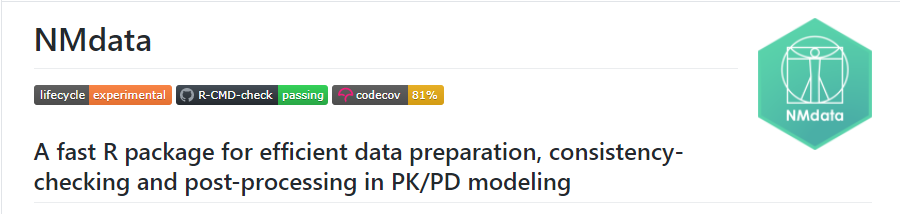
\includegraphics[width=.8\textwidth]{badges_snip_210623}

* `NMdata` contains very little calculations (only exception may be `flagsAssign`/`flagsCount`)

* Historic bugs have mostly resulted in uninformative errors due to
e.g. failure in processing text. Never a wrong data set.

* `NMdata` includes 190 "unit tests" where results of function calls
with different datasets and arguments are compared to expected
results

* Tests are consistently run before any release of the package

* The tests are crucial in making sure that fixing one bug or
introducing a new feature does not introduce new bugs

* The testing approach is as recommended in "R packages" by Hadley Wickham and Jennifer Bryan [https://r-pkgs.org/tests.html](https://r-pkgs.org/tests.html).

* If you have a specific example you want to make sure is tested in the
package, we will include the test in the package

# Next steps for `NMdata`
## Next steps for `NMdata`
* The following would be great help in making `NMdata` more accessible and useful
- Testing - please use the package and provide feedback
- Review of documentation, vignettes, and descriptions/explanations on website
- Graphical representations and illustrations.
- A tidyverse workflow for a new vignette
- If you have ideas you want to contribute, let's discuss!

* Additional features
- Functions to generate dosing regimens for simulations and
nominal-time datasets
- Functions for easy documentation of column contents (description,
units, 1:1 relationships between character and numeric columns)
- `NMfreezeModels`: Save Nonmem models with input data and all results to ensure reproducibility of output
<!-- %%%% automatic saving of meta data with csv files -->
<!-- %%%% check that row identifier is not modified by Nonmem -->
<!-- %%%% documentation of columnns -->

# Summary
::: columns
:::: column
Data creation

* `renameByContents` 
* `compareCols`
* `mergeCheck`
* `flagsAssign`/`flagsCount`
* `NMorderColumns`
* (`NMcheckData`)
* `NMwriteData`
* `NMstamp`/`NMinfo` 

Read/write Nonmem control streams

* `NMreadSection`/`NMwriteSection`
::::
:::: column
Retrieve data from Nonmem runs

* `NMscanData`
* `NMscanMultiple`
* `summary`, `NMinfo`
* `NMscanInput`, `NMreadCsv`
* `NMscanTables`, `NMreadTab`
* `NMcheckColnames`

Adjust behavior to your preferences

* `NMdataConf`

Other

* (`NMfreezeModels`)

:::: 
:::



# `NMdata` functions under development 




## NMfreezeModels

:::::::::::::: {.columns}
::: {.column width="85%"}
In order to ensure reproducibility, any output has to be produced based on arvhived/frozen Nonmem models. 
::: 
::: {.column width="15%"}

\includegraphics[width=.5in]{figures/worksign.png}
::: 
::::::::::::::

The components that need to be "frozen" are 

* Nonmem control streams
* input data
* estimation results (output tables, .lst, .ext etc.) 
* simulation code (say mrgsolve scripts)
* ?

`NMfreezeModels` does freeze

* input control streams
* input data
* all output tables
* all nonmem results files

Limitations

* NMfreezeModels does not provide a solution for the simulation code at this point. I am very interested in how we can do this.
* Only supports collections of models with one common input dataset
* The permissions of the frozen folder should be read-only. However,
that means that once the freeze it's done, you can no longer add
code or descriptions. It all has to be handled in the freeze
procedure.


## Safe model reader
:::::::::::::: {.columns}
::: {.column width="85%"}
* A function to read frozen Nonmem results and mrgsolve code to ensure that the right simulation model and parameter values are used

* Obviously, this is closely related to the way mrgsolve code is frozen together with nonmem code.
::: 
::: {.column width="15%"}

\includegraphics[width=.5in]{figures/ideabulb.jpg}
::: 
::::::::::::::


# Other tools
## tracee
* New package on CRAN from same author as `NMdata`
* A small package focusing on making outputs (graphics) traceable back to code
* The author has been using the code for years



## `ggwrite`: Flexible saving of tracable output
`ggwrite`: Saves images in sizes made for powerpoint, including stamps (time, source, output filename). It can save multiple plots at once as one file (pdf) or multiple files. 
::: columns
:::: column
`ggwrite` is a wrapper of `png` and `pdf` (and `dev.off`) with convenience features such as

* Support for multiple plots at once
- saved as either multiple files, named by list element names if wanted (or just numbered)
- or a single pdf with one plot per page
* Stamping with creation time, script name, and output name
* "canvas" sizes made for powerpoint or full-screen display (see `?canvasSize`)
* Custom canvases are very simple to create
* Independent `save` and `show` arguments for very simple conditional behavior
- `save` defaults to `TRUE` if a filename is given
- `show` defaults to the inverse of `save`
::::
:::: column
Save pls1, as one file and as multiple files, named by the dose levels.
\footnotesize
<!-- ```{r,warning=FALSE,message=FALSE,results=FALSE,fig.show="hide",eval=F} -->
<!-- writeOutput <- TRUE -->
<!-- script <- "path/to/script.R" -->
<!-- ggwrite(pls1,file="results/individual_profiles.png", -->
<!--         stamp=script,canvas="wide-screen",useNames=TRUE, -->
<!--         save=writeOutput) -->
<!-- ggwrite(pls1,file="results/individual_profiles.pdf", -->
<!--         stamp=script,canvas="wide-screen",useNames=TRUE, -->
<!--         save=writeOutput,onefile=TRUE) -->
<!-- list.files("results") -->
<!-- ``` -->
<!-- * Showing a bottom-right snip of `results/individual_profiles_trtact300mg.png`: -->
<!-- \begin{center} -->
<!-- 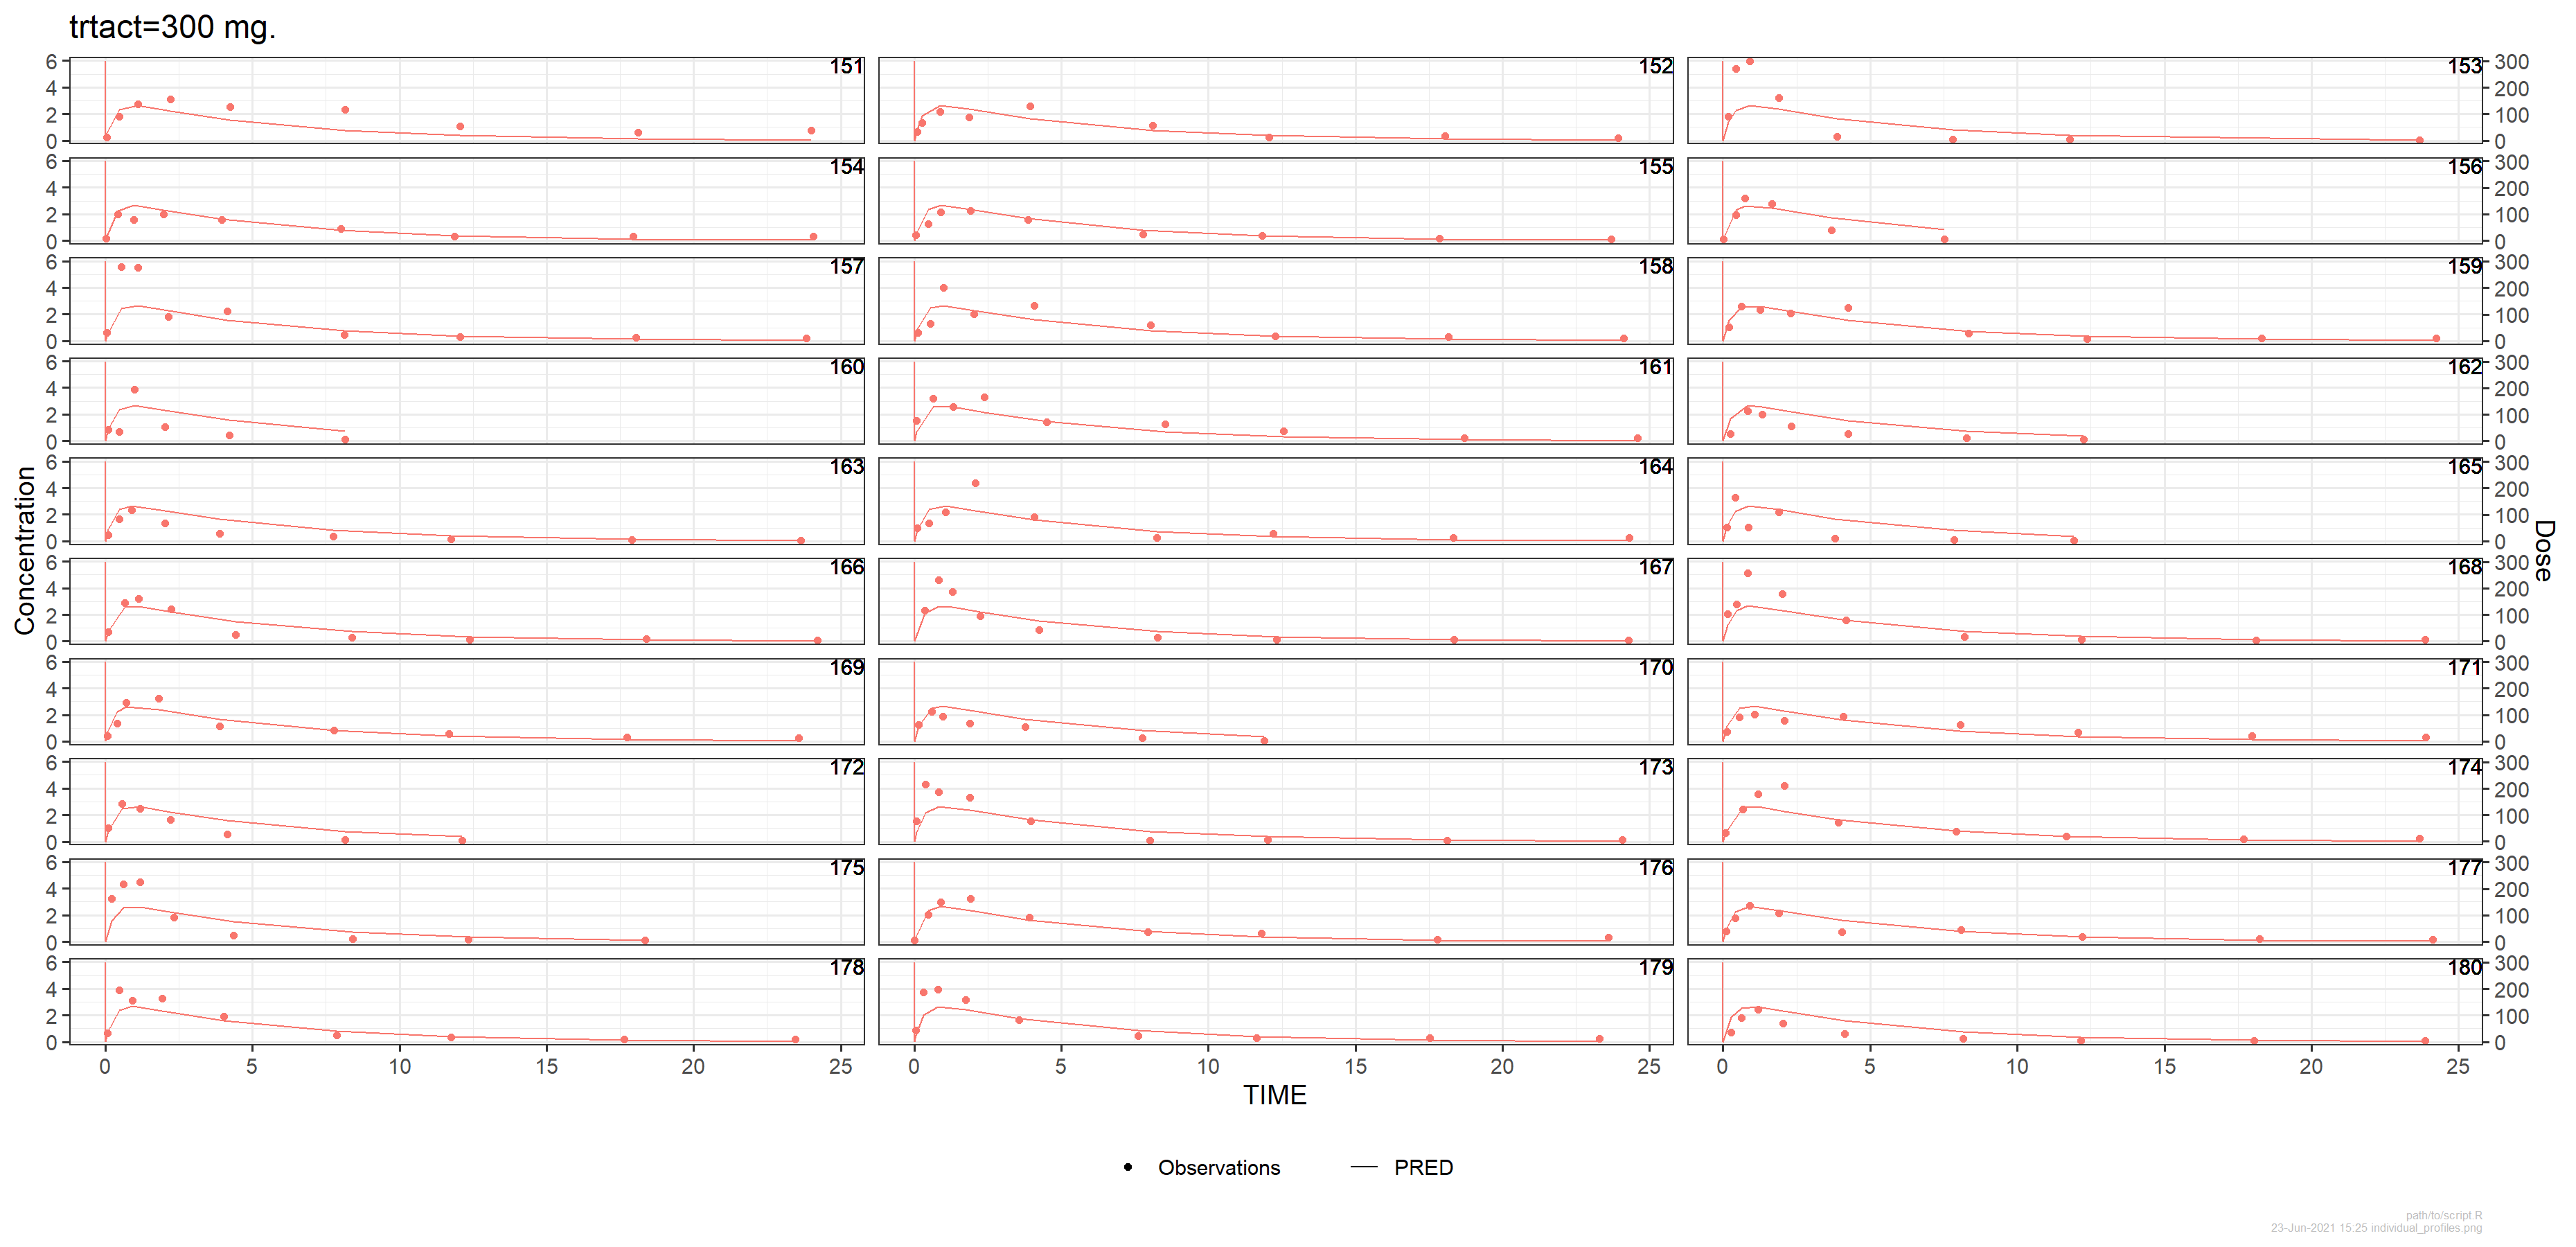
\includegraphics[trim={30cm 0 0 14cm},clip]{results/individual_profiles_trtact300mg.png} -->
<!-- \end{center} -->


```r
writeOutput <- TRUE
script <- "path/to/script.R"
p1 <- ggplot(res1,aes(PRED,DV,colour=TRTACT))+geom_point()+geom_abline(slope=1)+
    scale_x_log10()+scale_y_log10()
ggwrite(p1,file="results/pred_dv.png",
        stamp=script,
        save=writeOutput)
```
* Notice the caption with output and script file names.
\begin{center}
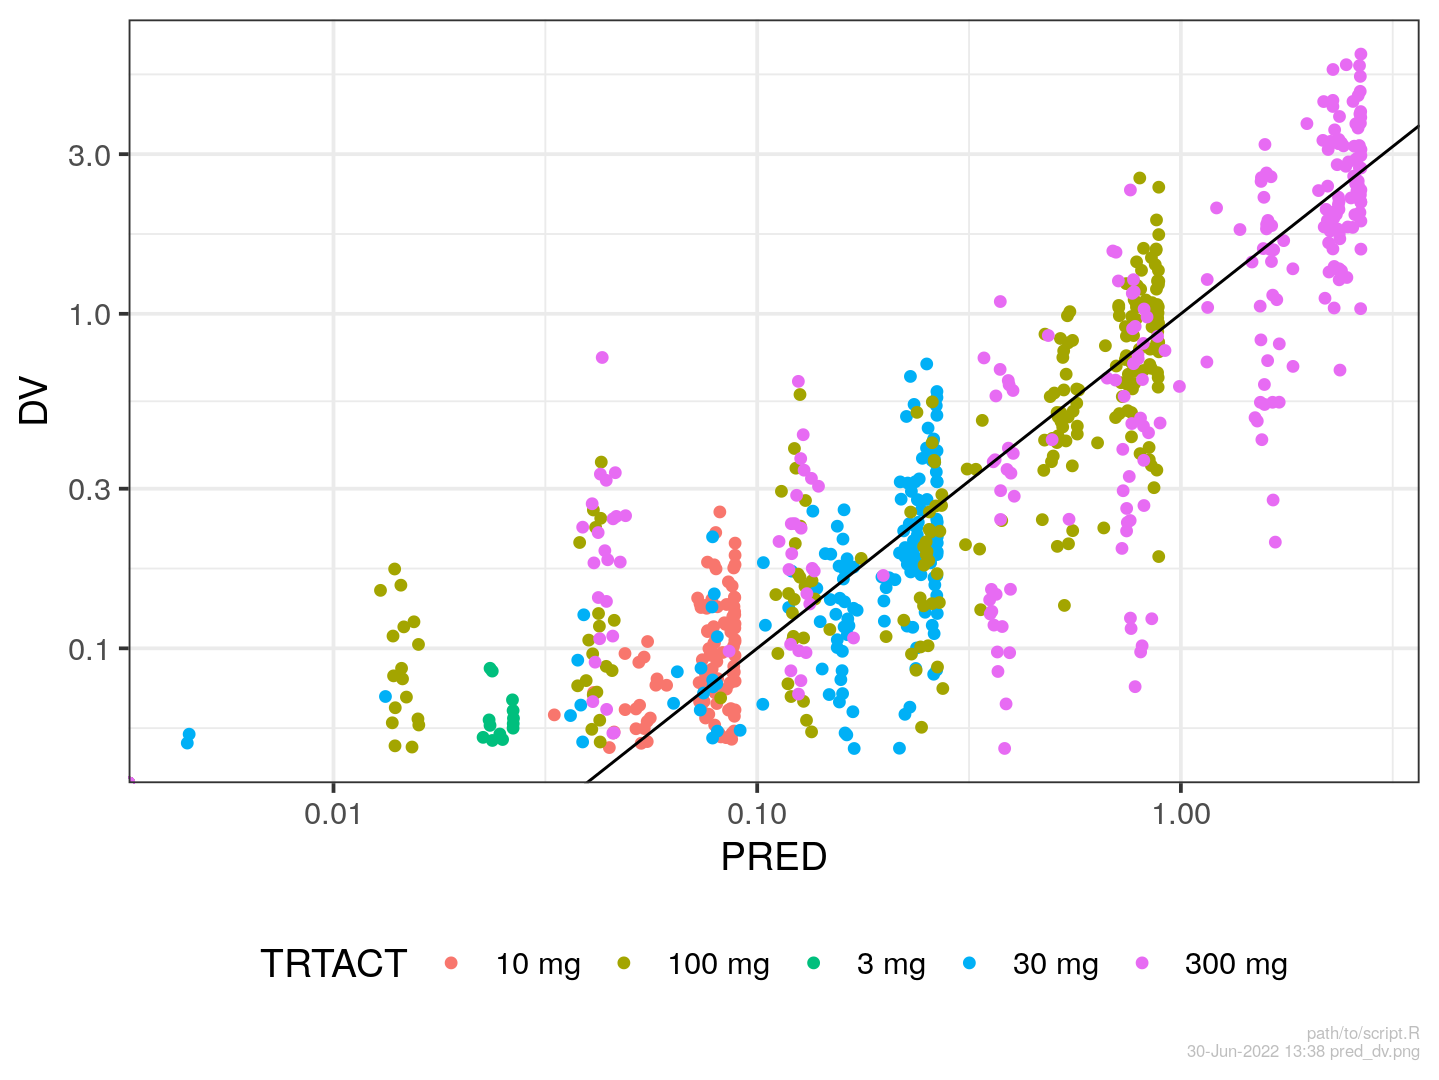
\includegraphics{results/pred_dv.png}
\end{center}


::::
:::

## `execSafe`: Save input data with each Nonmem run

* Executes Nonem from within R
* Archives input data together with Nonmem run (you can tell NMdata to read that archive when reading your model)
* Automatically generates a PNM file if you want to parallellize

